\documentclass[a4paper,12pt]{article} % [usenames] {article}

% ------------ Packages -------------

\usepackage[utf8]{inputenc}
\usepackage[spanish,es-tabla]{babel}
\usepackage[T1]{fontenc} 
\usepackage{anysize}    % Margins
\usepackage{fancyhdr}   % Headers and footers
\usepackage{caption,fixltx2e}
\usepackage[breaklinks]{hyperref}
%\usepackage{svg}
\usepackage{graphicx}
%\usepackage{subfigure}
%\usepackage{eurosym}
%\usepackage{amsmath}
%\usepackage{footnote}
%\usepackage{listings}
\usepackage{float}
\usepackage{color}
\usepackage{colortbl} % Colorear celdas
%\usepackage{hhline}
%\usepackage{multicol}
%\usepackage{multicolumn}
%\usepackage{multirow}
%\usepackage{framed}
\usepackage{courier}
\usepackage{indentfirst}
\usepackage{multicol}
\usepackage{verbatimbox}
\usepackage{graphicx}
\usepackage{cite}
\usepackage{subcaption}
\usepackage{neuralnetwork}
\usepackage{titlesec}
\usepackage{booktabs}
\usepackage{enumitem}
\usepackage[font=scriptsize,labelfont=bf]{caption}
\usepackage[font=scriptsize,labelfont=bf]{subcaption}
\newcommand{\tableref}[1]{\textit{tabla \ref{#1}}}
\newcommand{\figureref}[1]{\textit{figura \ref{#1}}}


% ------------- Style ---------------

\hypersetup{
	colorlinks   = true,	% Colours links instead of ugly boxes
	urlcolor     = black,	% Colour for external hyperlinks
	linkcolor    = black,	% Colour of internal links
	citecolor   = black		% Colour of citations
}

\marginsize{2.25cm}{2.25cm}{2cm}{2cm}
\setlength{\parskip}{\baselineskip}
% Make numbering begins at 1, not at 0.
\renewcommand{\thesection}{\arabic{section}}
%\addto\captionsspanish{\renewcommand{\chaptername}{Practice}}
\definecolor{LightCyan}{rgb}{0.88,1,1}

\renewcommand\labelitemi{\scriptsize$\bullet$} %Set bullets as default item symbol
\AtBeginDocument{\addtocontents{toc}{\protect\thispagestyle{empty}}}



\setcounter{secnumdepth}{4}

\titleformat{\paragraph}
{\normalfont\normalsize\bfseries}{\theparagraph}{1em}{}
\titlespacing*{\paragraph}
{0pt}{3.25ex plus 1ex minus .2ex}{1.5ex plus .2ex}


% ------- NewCommand -------
\newcommand{\tab}{\indent}




% ------- Variables -------
\def \frontTitle {Lógica difusa}
\def \authorOne {Eva Suárez García\\eva.suarez.garcia@udc.es}
\def \authorTwo {Rafael Alcalde Azpiazu\\rafael.alcalde.azpiazu@udc.es}
\def \authorThree {Iago Otero Coto\\iago.oteroc@udc.es}
\def \authorFour {Manuel José Rivas Fariñas\\manuel.rivasf@udc.es}


\def \subject {Razonamiento Automático}
\def \course {3º Grado en Ingeniería Informática \\ Mención de Computación }
\def \place {A Coruña } 

% ------- Document -------

\begin{document}
	
	% ------- TitlePage -------
	
	\begin{titlepage}
   	\thispagestyle{empty}
   	\begin{center}
   		{
	   		\vspace*{\fill}
	   		\textbf{
\includegraphics[scale=0.4]{images/Portada/udc.png}}\\[2cm]
	   		{\Large \subject}\\[1.5cm]
	   		{\LARGE \textbf{\frontTitle}}\\[2cm]
	   			   	
		   	
		   	\begin{multicols}{2}
		   		\begin{flushleft}
		   			\centering{\authorOne} \\
		   			\vspace{0.5cm}
		   			\centering{\authorThree} \\
		   			\vspace{0.5cm}	   		
		   		\end{flushleft} 
		   		
		   		\columnbreak 
		   		
		   		\begin{flushleft}
		   			\centering{\authorTwo} \\
		   			\vspace{0.5cm}
		   			\centering{\authorFour} \\
		   			\vspace{0.5cm}	   		
		   		\end{flushleft} 
		   	\end{multicols}
		   	
		   	\vfill
	  
	   		
	   		\course\\[0.25cm]
	   		\place - \today \\[1.25cm]
	   		\vspace*{\fill}
    	}
   	\end{center}
\end{titlepage}
	\newpage
	\thispagestyle{empty}
	
	% ------- Index -------
	
	\tableofcontents
	
	% ------- Style -------
	\newpage
	\setcounter{page}{1}
	\pagestyle{plain} %{plain}
	
	\hypersetup{
		linkcolor = black, % Colour of internal links
	}



	% ------- Content -------
	\input{introducción}
	\input{introducción_y_objetivos}
	\newpage
	\section{Fundamentos de los sistemas difusos.}

\subsection{Introducción}
En los últimos años se han consolidado y aumentado las aplicaciones de la lógica difusa, abarcando sectores tan diversos como puede ser el control industrial, las búsquedas en bases de datos o estrategias de mantenimiento entre otros.

Las principales razones para tal proliferación de aplicaciones quizás sean la
sencillez conceptual de los Sistemas basados en Lógica Difusa, su facilidad
para adaptarse a casos particulares con pocas variaciones de parámetros,
su habilidad para combinar en forma unificada expresiones lingüísticas con
datos numéricos, y el no requerir de algoritmos muy sofisticados para su
implementación.

La lógica tradicional (así como la teoría de conjuntos y el algebra booleana) son isomorfas\footnote{\url{http://matematica.laguia2000.com/general/isomorfismo}}, bajo transformaciones adecuadas, es decir, tienen una estructura similar, lo cual significa que, las definiciones hechas para cualquiera de las tres teorías se pueden llevar a las otras dos mediante transformaciones sencillas, mediante la correspondencia de operadores que se muestra en la \tableref{table:1}.



\begin{table}[h]
	\centering
	\begin{tabular}{@{}ccc@{}}
		\toprule
		\multicolumn{1}{l}{\textbf{Teoría de conjuntos}} & \multicolumn{1}{l}{\textbf{Álgebra booleana}} & \multicolumn{1}{l}{\textbf{Lógica tradicional}} \\ \midrule
		\multicolumn{1}{c}{Intersección}               & \multicolumn{1}{c}{Conjunción}               & \multicolumn{1}{c}{AND}                        \\ \midrule
		\multicolumn{1}{c}{Unión}                      & \multicolumn{1}{c}{Disyunción}               & \multicolumn{1}{c}{OR}                         \\ \midrule
		Complemento                                      & Negación                                      & NOT                                             \\ \bottomrule
	\end{tabular}
	\caption{Correspondencia entre operadores de la Teoría de Conjuntos, el Álgebra Booleana y la Lógica Tradicional.}
	\label{table:1}
\end{table}

\subsection{Teoría de conjuntos difusos}
Antes de comenzar con la definición de Conjuntos Difusos, veamos cómo se definen los conjuntos convencionales (Conjuntos Concretos).

Un conjunto concreto se define como una colección de elementos que
existen dentro de un Universo. Así, dado el universo U que consta de los números enteros no negativos menores que 10:

\texttt{U = \{0,1,2,3,4,5,6,7,8,9\}}

podemos definir algunos conjuntos como\\
\newline
\null\hspace{0.59cm}\texttt{A = \{0,2,4,6,8\}},\newline
\null\hspace{0.37cm}\texttt{ B=\{1,3,5,7,9\}},\newline
\null\hspace{0.37cm}\texttt{ C=\{1,4,7\}} \ldots

De esta forma, hemos establecido a qué conjuntos pertenecen cada uno de los elementos del universo \texttt{U}. Cada uno de estos conjuntos queda perfectamente definido si utilizamos una función de pertenencia (\texttt{u(x)}) sobre los elementos del universo \texttt{U} de forma que, a cada elemento de \texttt{U} se le asigna un valor 1 o 0 si pertenece o no a dicho conjunto.

Veamos como ejemplo la función de pertenencia que define el conjunto \texttt{C}
\\ \newline
\null\hspace{0.59cm}\texttt{u\textsubscript{C}(0)} = 0;\\
\null\hspace{0.59cm}\texttt{u\textsubscript{C}(1)} = 1;\\
\null\hspace{0.59cm}\texttt{u\textsubscript{C}(2)} = 0;\\
\null\hspace{0.59cm}\texttt{u\textsubscript{C}(3)} = 0;\\
\null\hspace{0.59cm}\texttt{u\textsubscript{C}(4)} = 1;\\
\null\hspace{0.59cm}\texttt{u\textsubscript{C}(5)} = 0;\\
\null\hspace{0.59cm}\texttt{u\textsubscript{C}(6)} = 0;\\
\null\hspace{0.59cm}\texttt{u\textsubscript{C}(7)} = 1;\\
\null\hspace{0.59cm}\texttt{u\textsubscript{C}(8)} = 0;\\
\null\hspace{0.59cm}\texttt{u\textsubscript{C}(9)} = 0;

Un Conjunto difuso se define de forma similar, con una diferencia conceptual importante: un elemento puede pertenecer parcialmente a un conjunto.
Pues bien, un Conjunto Difuso se define de forma similar, con una
diferencia conceptual importante: un elemento puede pertenecer
parcialmente a un conjunto. 

Continuemos con el universo \texttt{U} que definimos anteriormente.
Un conjunto difuso D definido sobre dicho universo podría ser el siguiente:
\\ \newline
\null\hspace{0.59cm}\texttt{C=\{20\%/1,50\%/4,100\%/7\}}

Con esta definición, estamos representando que el elemento 1 pertenece en un 20\% al
conjunto \texttt{C} (y por tanto pertenece en un 80\% al complemento de \texttt{C}), mientras que
que el elemento 4 pertenece en un 50\%, y el elemento 7 en un 100\% .

De igual forma que con los Conjuntos Concretos, podemos definir una función de pertenencia \texttt{u\textsubscript{C}(x)}:
\\ \newline
\null\hspace{0.59cm}\texttt{u\textsubscript{C}(0)} = 0.0;\\
\null\hspace{0.59cm}\texttt{u\textsubscript{C}(1)} = 0.2;\\
\null\hspace{0.59cm}\texttt{u\textsubscript{C}(2)} = 0.0;\\
\null\hspace{0.59cm}\texttt{u\textsubscript{C}(3)} = 0.0;\\
\null\hspace{0.59cm}\texttt{u\textsubscript{C}(4)} = 0.5;\\
\null\hspace{0.59cm}\texttt{u\textsubscript{C}(5)} = 0.0;\\
\null\hspace{0.59cm}\texttt{u\textsubscript{C}(6)} = 0.0;\\
\null\hspace{0.59cm}\texttt{u\textsubscript{C}(7)} = 1.0;\\
\null\hspace{0.59cm}\texttt{u\textsubscript{C}(8)} = 0.0;\\
\null\hspace{0.59cm}\texttt{u\textsubscript{C}(9)} = 0.0;

Como podemos ver, hay algunas diferencias sustanciales entre los Conjuntos Difusos y los Conjuntos Concretos:
\begin{itemize}
	\item La función de pertenencia asociada a los Conjuntos Concretos sólo puede
	tener dos valores: 1 ó 0, mientras que en los conjuntos difusos puede
	tener cualquier valor entre 0 y 1.
	\item Un elemento puede pertenecer (parcialmente) a un conjunto difuso y
	simultáneamente pertenecer (parcialmente) al complemento de dicho
	conjunto. Esto no es posible en los conjuntos concretos, ya que
	constituiría una violación al \textit{principio del tercer excluido.}\footnote{\url{https://es.wikipedia.org/wiki/Principio_del_tercero_excluido}}
	\item Las fronteras de un conjunto concreto son exactas, en tanto que las de
	un conjunto difuso son, precisamente, difusas, ya que existen elementos
	en las fronteras mismas, y estos elementos están a la vez dentro y fuera
	del conjunto.
\end{itemize}

En el mundo real, el hecho de que un elemento pueda pertenecer parcialmente a un conjunto tiene numerosas ventajas, veamos un ejemplo;

\textit{Ejemplo 1:} Supóngase que se desea clasificar a los miembros de un equipo
de fútbol según su estatura en tres conjuntos, Bajos, Medianos y Altos.
Podría plantearse que se es Bajo si se tiene una estatura inferior a, por
ejemplo, 160 cm, que se es Mediano si la estatura es superior o igual a 160
cm e inferior a 180 cm, y se es alto si la estatura es superior o igual a 180
cm, con lo que se lograría una clasificación en conjuntos concretos. \label{ej:1}

Si embargo, es tan significativa la diferencia entre un jugador con estatura 179.9 cm y otro de 180 cm? Ese milímetro representa una diferencia tan significativa que tenemos que clasificar a los jugadores en dos conjuntos distintos? Utilizando Conjuntos Categóricos uno es alto y otro es mediano.

Si se optase por efectuar la misma
clasificación con conjuntos difusos estos cambios abruptos se evitarían,
debido a que las fronteras entre los conjuntos permitirían cambios graduales
en la clasificación.

\begin{figure}[H]
	\centering
	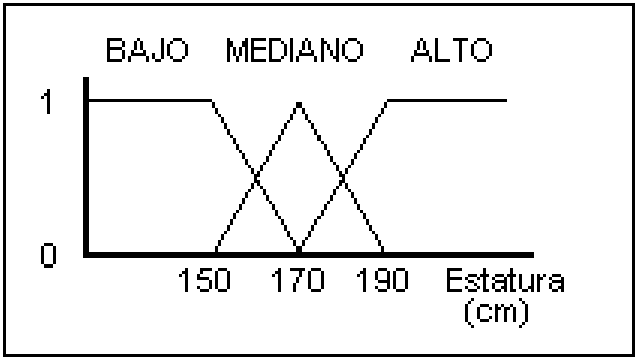
\includegraphics[scale=0.3]{images/fuzzy_example.png}
	\caption{Funciones de pertenencia del ejemplo 1}
	\label{fig:ej1}
\end{figure}
La \figureref{fig:ej1} muestra cómo podría hacerse dicha clasificación: el universo de
discurso sería el conjunto continuo de todas las posibles estaturas (el
intervalo [130,210]cm por ejemplo). 

\begin{figure}[H]
	\centering
	\begin{subfigure}[b]{0.4\textwidth}
		\centering
		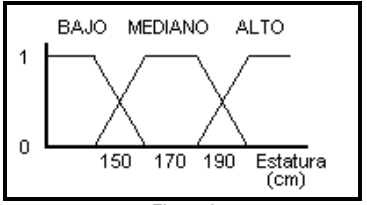
\includegraphics[scale = 0.5]{images/fuzzy_example_alt1.png}
		\caption{Representación alternativa del ejemplo 1}
		\label{fig:fuzzy1}
	\end{subfigure}
	~ %add desired spacing between images, e. g. ~, \quad, \qquad, \hfill etc. 
	%(or a blank line to force the subfigure onto a new line)
	\begin{subfigure}[b]{0.4\textwidth}
		\centering
		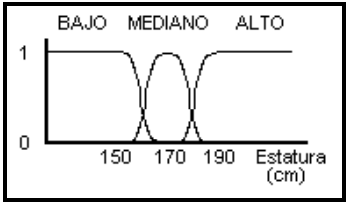
\includegraphics[scale = 0.5]{images/fuzzy_example_alt2.png}
		\caption{Representación alternativa del ejemplo 1}
		\label{fig:fuzzy2}
	\end{subfigure}
	\label{fig:alternativas}	
\end{figure}
La forma de
estas funciones de pertenencia no debe ser necesariamente la de la \figureref{fig:ej1} ,
pues depende de lo que se entienda por ``Bajo'', ``Mediano'' y ``Alto''.
En las \textit{figuras \ref{fig:fuzzy1} y \ref{fig:fuzzy2}} podemos ver otras alternativas para representar dichas funciones.

\subsection{Inferencia en lógica difusa}
La Inferencia lógica consiste en la combinación de proposiciones para
producir nuevas proposiciones. Así, al combinar la proposición \texttt{``X es A''} con
la proposición \texttt{``IF X es A THEN Y es B''}, se puede inferir la proposición \texttt{``Y es
B''} (ver figura \figureref{fig:inf})

\begin{figure}[H]
	\centering
	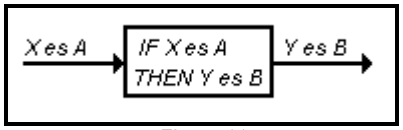
\includegraphics[scale=0.5]{images/logica_difusa.png}
	\caption{Inferencia en lógica tradicional.}
	\label{fig:inf}
\end{figure}

Una inferencia como ésta sólo es posible en
la lógica tradicional si la primera proposición \texttt{(``X es A'')} es idéntica a la
primera parte de la segunda proposición \texttt{(``(IF) X es A'')}; sin embargo, en la
lógica difusa estas dos proposiciones no necesariamente deben ser
idénticas, debido a que las fronteras de los conjuntos no son precisas. Así, al
combinar la proposición \texttt{``X es A*''} con la proposición \texttt{``IF X es A THEN Y es
B''}, puede obtenerse la proposición \texttt{``Y es B*''} (ver figura \figureref{fig:inf}).

\begin{figure}[H]
	\centering
	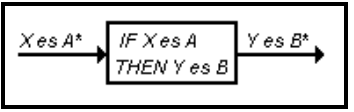
\includegraphics[scale=0.67]{images/logica_difusa_1.png}
	\caption{Inferencia en lógica difusa.}
	\label{fig:inf1}
\end{figure}

En la \figureref{fig:inferencia} podemos ver los mecanismos de Inferencia en Lógica Difusa \footnote{\url{http://www.cs.princeton.edu/courses/archive/fall07/cos436/HIDDEN/Knapp/fuzzy004.htm}}

\begin{figure}[H]
	\centering
	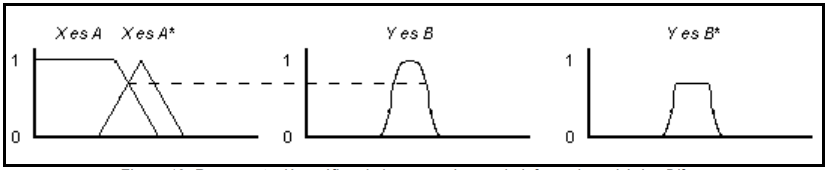
\includegraphics[scale=0.67]{images/mecanismos_inferencias_logica_difusa.png}
	\caption{Representación gráfica de los mecanismos de Inferencia en Lógica Difusa}
	\label{fig:inferencia}
\end{figure}

\subsection{Sistemas de lógica difusa}
Los mecanismos de Inferencia permiten
obtener Conjuntos difusos a partir de la combinación de Conjuntos difusos
con reglas de la forma \texttt{IF... THEN...}; un Sistema de Lógica Difusa aprovecha
esos mecanismos como el motor de cálculo de un sistema cuyas entradas y
salidas son números concretos.

En la \figureref{fig:sistemas_difusos} podemos ver la estructura básica de un Sistema de Lógica difusa.
El sistema recibe varias entradas numéricas y entrega varias salidas
numéricas. El bloque Difusor se encarga de convertir las entradas en
conjuntos difusos, que son entregados al bloque Máquina de Inferencia que, utilizando las reglas de la forma \texttt{IF... THEN...} almacenadas en la Base de Reglas  este, produce varios conjuntos difusos para
que el bloque Concresor los tome y los convierta en salidas numéricas
concretas.
\begin{figure}[H]
	\centering
	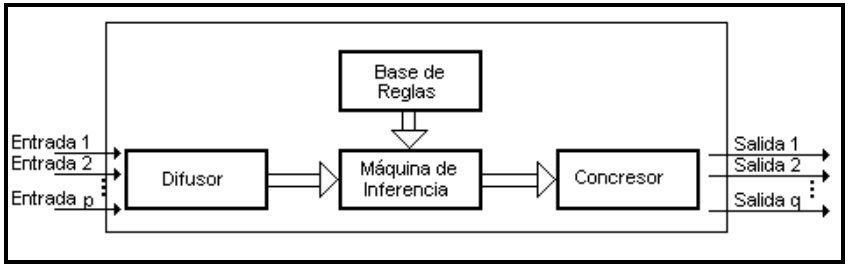
\includegraphics[scale=0.67]{images/sistemas_difusos.png}
	\caption{Estructura de un Sistema de Lógica Difusa}
	\label{fig:sistemas_difusos}
\end{figure}


Cada una de las variables de entrada y de salida tiene una representación
dentro del Sistema de Lógica Difusa en forma de Variables Lingüísticas. Una
variable lingüística tiene, entre otras cosas, una colección de atributos que
puede adquirir la variable, y cada atributo está representado por un conjunto
difuso. Así, retomando el ejemplo de la \figureref{fig:ej1}, la variable Estatura tendría
tres atributos, Bajo, Mediano y Alto, y cada uno de estos atributos estaría
representado por el conjunto difuso respectivo de la \figureref{fig:ej1}. Estos atributos
reciben el nombre de Valores Lingüísticos.
	\newpage
	\input{metodología}
	\newpage
	\section{Casos de uso}

Para comprobar el correcto funcionamiento del sistema desarrollado, hemos establecido una serie de casos de prueba representativos que se muestran a continuación:

\begin{figure}[H]
	\centering
	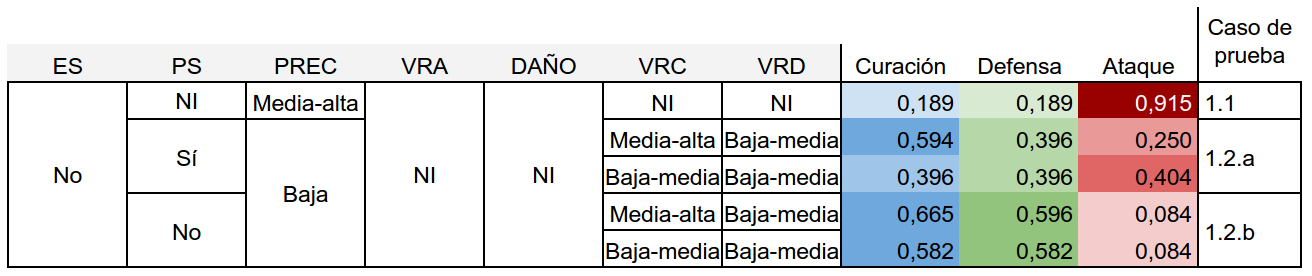
\includegraphics[width=\textwidth,height=\textheight,keepaspectratio]{images/casos_pruebas.png}
	\caption{Casos de prueba 1}
	\label{fig:casos_prueba1}
\end{figure}

\begin{figure}[H]
	\centering
	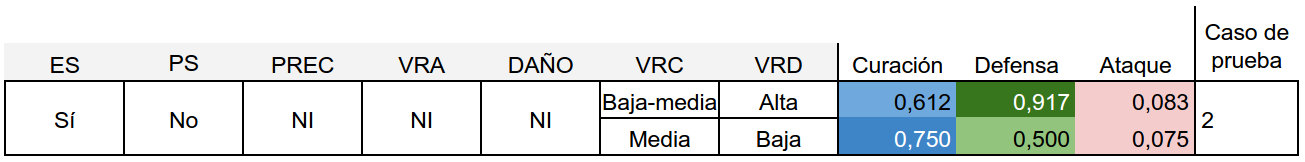
\includegraphics[width=\textwidth,height=\textheight,keepaspectratio]{images/casos_pruebas1.png}
	\caption{Casos de prueba 2}
	\label{fig:casos_prueba2}
\end{figure}


\begin{figure}[H]
	\centering
	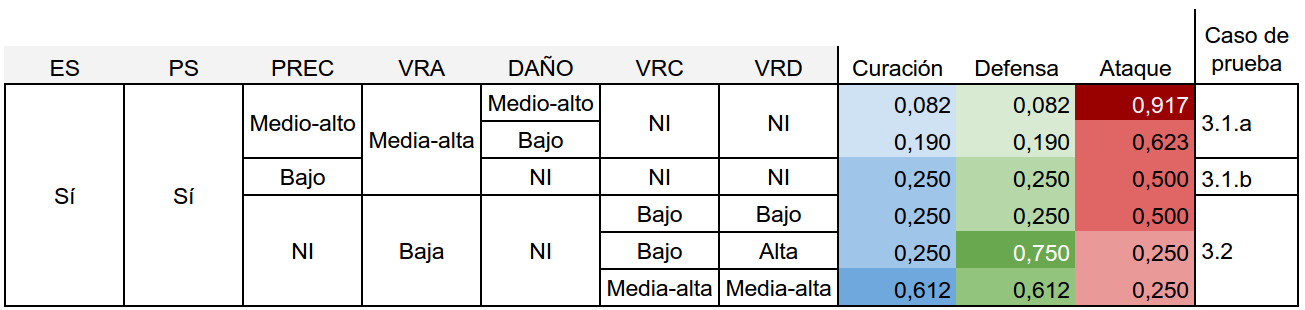
\includegraphics[width=\textwidth,height=\textheight,keepaspectratio]{images/casos_pruebas2.png}
	\caption{Casos de prueba 3}
	\label{fig:casos_prueba3}
\end{figure}
Hemos elegido dividirlos en tres grupos:
\begin{enumerate}
	\item El enemigo no sobrevive al ataque.
	\item El enemigo sobrevive al ataque pero nuestro personaje no.
	\item El enemigo sobrevive y nuestro personaje también.
\end{enumerate}


\begin{enumerate}
	
	\item En el primer grupo, hemos elegido dos casos representativos, uno de los cuales se subdivide:
	\begin{enumerate}[label={1.\arabic*.}]
		\item La precisión es media-alta. Teniendo esto en cuenta, es fácil decidir que lo mejor es atacar, ya que el enemigo es muy probable que no sobreviva al ataque y por tanto el combate terminaría en una victoria. Como se puede observar en la tabla, el sistema devuelve un resultado coherente con el anterior razonamiento, dándole al Ataque una adecuación del 0,915, mientras que a Curación y Defensa sólamente un 0,189.
		\item La precisión es baja. En este caso debemos fijarnos en si el personaje sobreviviría o no al fallar el ataque, por lo que dividimos este caso en dos subcasos:
		\begin{enumerate}[label=\alph*)]
			\item El personaje sobrevive. Sabiendo esto, debemos comprobar la vida restante al defenderse y al curarse. Si suponen una mejora lo suficientemente importante, la Curación o la Defensa tendrán más adecuación que el Ataque. Se puede observar que los resultados arrojados por el sistema son coherentes.
			\item El personaje no sobrevive. Como es lógico, en este caso debemos pensar en Curación y Defensa como las opciones más viables y optar por una o la otra en función de la vida restante al realizar cada una de ellas. De nuevo, el sistema devuelve unos resultados razonables.
		\end{enumerate}
	\end{enumerate}
\item El segundo grupo se asemeja al caso 1.2.b del primer grupo. Nuestro personaje no sobrevive al ataque, por lo que debe centrarse en Curación o Defensa. Igual que en el 2.b, debemos decidir en función de la vida restante, y seguimos obteniendo resultados lógicos.

\item El último grupo es algo más complicado, ya que se deben tener en cuenta más factores para poder realizar una acción óptima, como el daño que vamos a realizar y la vida restante después de realizar un ataque. Podemos distinguir dos casos representativos, que a su vez se dividen en subcasos:
\begin{enumerate}[label={3.\arabic*.}]
	\item La vida restante del personaje después de atacar es media-alta. Podemos centrarnos ahora en decidir con cuánta adecuación atacamos, ya que la Curación y Defensa nos privarían de una buena oportunidad para atacar:
	\begin{enumerate}[label=\alph*)]
		\item La precisión es media-alta. Para tener un mejor criterio, nos ayudamos de la variable de entrada DAÑO. Con un daño medio-alto, la adecuación del Ataque debe ser muy alta y la de Curación y Defensa muy baja. Con un daño bajo, el Ataque seguiría siendo una buena opción aunque con peor adecuación. Los resultados al establecer estos datos en el sistema, concuerdan con el razonamiento que hemos llevado a cabo.
		\item La precisión es baja. En este caso no es necesario tener en cuenta ninguna otra variable. El Ataque es medianamente adecuado y la Curación y Defensa deben ganar algo de adecuación, aunque sin superar el Ataque. Como podemos observar, los datos obtenidos vuelven a ser razonables.
	\end{enumerate}
	\item La vida restante del personaje después de atacar es baja. Debemos tener cuidado, por lo que decidimos la adecuación de las tres opciones en función de la vida restante después de curarse y después de defenderse. Si ambas son tan bajas como la vida restante después de atacar, el ataque es la mejor opción. Sin embargo, en caso contrario, la adecuación será mayor para Curarse o Defenderse, dependiendo de la cantidad de vida restante en cada caso. Los resultados del sistema siguen, de nuevo, el razonamiento llevado a cabo.
\end{enumerate}
\end{enumerate}
	\newpage
	\section{Discusión.}
	\newpage
	\section{Referencias}


[1] Carlos González Morcillo,  \textit{Lógica Difusa
Una introducción práctica
Técnicas de Softcomputing}, 2011


[2] Oscar G. Duarte V. M.Sc., \textit{Sistemas de Lógica Difusa }
	
	
\end{document}